% Unterstützung für Links und PDF Metadaten
\documentclass[
  bibliography=totoc,     % Literatur im Inhaltsverzeichnis
  captions=tableheading,  % Tabellenüberschriften
  titlepage=firstiscover, % Titelseite ist Deckblatt
]{scrartcl}

% Paket float verbessern
\usepackage{scrhack}

% Warnung, falls nochmal kompiliert werden muss
\usepackage[aux]{rerunfilecheck}

% unverzichtbare Mathe-Befehle
\usepackage{amsmath}
% viele Mathe-Symbole
\usepackage{amssymb}
% Erweiterungen für amsmath
\usepackage{mathtools}

% Fonteinstellungen
\usepackage{fontspec}
% Latin Modern Fonts werden automatisch geladen
% Alternativ zum Beispiel:
%\setromanfont{Libertinus Serif}
%\setsansfont{Libertinus Sans}
%\setmonofont{Libertinus Mono}

% Wenn man andere Schriftarten gesetzt hat,
% sollte man das Seiten-Layout neu berechnen lassen
\recalctypearea{}

% deutsche Spracheinstellungen
\usepackage{polyglossia}
\setmainlanguage{german}


\usepackage[
  math-style=ISO,    % ┐
  bold-style=ISO,    % │
  sans-style=italic, % │ ISO-Standard folgen
  nabla=upright,     % │
  partial=upright,   % ┘
  warnings-off={           % ┐
    mathtools-colon,       % │ unnötige Warnungen ausschalten
    mathtools-overbracket, % │
  },                       % ┘
]{unicode-math}

% traditionelle Fonts für Mathematik
\setmathfont{Latin Modern Math}
% Alternativ zum Beispiel:
%\setmathfont{Libertinus Math}

\setmathfont{XITS Math}[range={scr, bfscr}]
\setmathfont{XITS Math}[range={cal, bfcal}, StylisticSet=1]

% Zahlen und Einheiten
\usepackage[
  locale=DE,                   % deutsche Einstellungen
  separate-uncertainty=true,   % immer Fehler mit \pm
  per-mode=symbol-or-fraction, % / in inline math, fraction in display math
]{siunitx}

% chemische Formeln
\usepackage[
  version=4,
  math-greek=default, % ┐ mit unicode-math zusammenarbeiten
  text-greek=default, % ┘
]{mhchem}

% richtige Anführungszeichen
\usepackage[autostyle]{csquotes}

% schöne Brüche im Text
\usepackage{xfrac}

% Standardplatzierung für Floats einstellen
\usepackage{float}
\floatplacement{figure}{htbp}
\floatplacement{table}{htbp}

% Floats innerhalb einer Section halten
\usepackage[
  section, % Floats innerhalb der Section halten
  below,   % unterhalb der Section aber auf der selben Seite ist ok
]{placeins}

% Seite drehen für breite Tabellen: landscape Umgebung
\usepackage{pdflscape}

% Captions schöner machen.
\usepackage[
  labelfont=bf,        % Tabelle x: Abbildung y: ist jetzt fett
  font=small,          % Schrift etwas kleiner als Dokument
  width=0.9\textwidth, % maximale Breite einer Caption schmaler
]{caption}
% subfigure, subtable, subref
\usepackage{subcaption}

% Grafiken können eingebunden werden
\usepackage{graphicx}
% größere Variation von Dateinamen möglich
\usepackage{grffile}

% schöne Tabellen
\usepackage{booktabs}

% Verbesserungen am Schriftbild
\usepackage{microtype}

% Literaturverzeichnis
\usepackage[
  backend=biber,
]{biblatex}
% Quellendatenbank
\addbibresource{lit.bib}
\addbibresource{programme.bib}

% Hyperlinks im Dokument
\usepackage[
  unicode,        % Unicode in PDF-Attributen erlauben
  pdfusetitle,    % Titel, Autoren und Datum als PDF-Attribute
  pdfcreator={},  % ┐ PDF-Attribute säubern
  pdfproducer={}, % ┘
]{hyperref}
% erweiterte Bookmarks im PDF
\usepackage{bookmark}

% Trennung von Wörtern mit Strichen
\usepackage[shortcuts]{extdash}

\usepackage{tikz}
\usepackage{tikzscale}
\usetikzlibrary{arrows.meta}

\author{%
  Judith Gnade\\%
  \href{mailto:judith.gnade@tu-dortmund.de}{judith.gnade@tu-dortmund.de}%
  \texorpdfstring{\and}{,}%
  Yascha Franz\\%
  \href{mailto:yascha.franz@tu-dortmund.de}{yascha.franz@tu-dortmund.de}%
}
\publishers{TU Dortmund – Fakultät Physik}

% Einstellungen hier, z.B. Fonts



\begin{document}
% Text hier
\title{V27 – Zeeman-Effekt}
\date{Durchführung: 08.01.2020, Abgabe: 19.01.2020}

% 7 \, s vor Korrekturabgabe:

\maketitle
\tableofcontents
\newpage

\section{Zielsetzung und Theorie}

\subsection{Zielsetzung}
Es wird die Dipolrelaxation in Ionenkristallen untersucht. Dabei sollen die charakteristische
Relaxationszeit der Dipole sowie die Aktivierungsenergie bestimmt werden.


\subsection{Theorie}
Laser sind in der Lage Licht mit einer besonders hohen Intensität zu erzeugen. Der Lichtstrahl ist dabei sehr stark fokussiert,
die elektromagnetischen Wellen besitzen die gleiche Frequenz und sind kohärent zueinander. Die Prozesse, die zur
Erzeugung des Laserlichts führen, finden im Wesentlichen in drei verschiedenen Komponenten des Lasers statt.

\begin{figure}
\centering
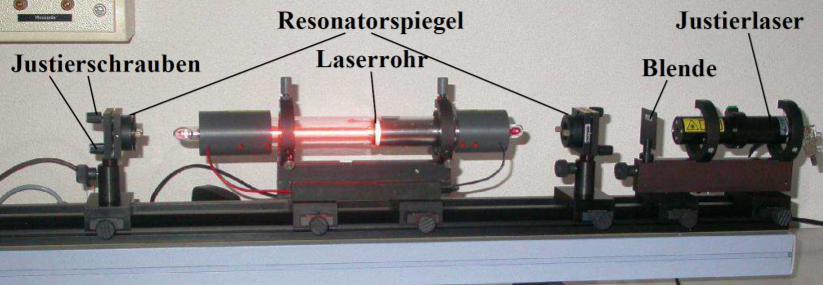
\includegraphics[width=\textwidth]{laseraufbau.png}
\caption{Aufbau eines He-Ne-Lasers.\cite[3]{anleitung}}
\label{fig:laseraufbau}
\end{figure}

\subsection{Der Resonator}

Der Resonator besteht aus zwei Spiegeln, zwischen denen sich ein Glasrohr befindet. Dieses ist mit einem Helium-Neon-Gasgemisch
gefüllt. Die Spiegel sind dabei hochreflektierend, lassen jedoch auch einen kleinen Teil des Lichtes hindurch, sodass das
Laserlicht aus dem Resonator austreten kann. Sie können unterschiedliche Krümmungsradien haben (konkav oder plan-parallel).

Im Resonator bilden sich nur unter bestimmten Voraussetzungen stehende Wellen aus, die dann verstärkt werden können.
Andere Wellen werden aufgrund destruktiver Interferenzen stark abgeschwächt. Nur wenn die Länge des Resonators durch ein
Vielfaches der halben Wellenlänge teilbar ist, überlagern sich die Wellen auf optimale Weise und das Licht wird gut verstärkt.

Links und rechts des Resonators sind außerdem noch Brewsterfenster angebracht, die dafür sorgen dass das emittierte Licht
parallel-polarisiert ist. Die Fenster stehen im Brewster-Winkel zur optischen Achse, sodass senkrecht-polarisiertes
Licht herausgefiltert und das Licht in Ausbreitungsrichtung verstärkt wird.

Ein Resonator gilt als stabil, wenn seine Verluste möglichst gering sind und die Verstärkung des Lichts gut funktionniert.
Die Bedingung für Stabilität ist dabei durch den Stabilitätsparameter $g_1g_2$ gegeben. Er sollte zwischen 0 und 1 liegen.

\begin{equation}
  g_1g_2 = \biggl(1-\frac{L}{R_1}\biggr)\biggl(1-\frac{L}{R_2}\biggr)
\end{equation}

($L$: Länge des Resonators bzw. Abstand zwischen den Spiegeln, $R_1$,$R_2$: Krümmungsradien der beiden Spiegel des Resonators)

\subsection{Das verstärkende Medium}

Im Glasrohr des Lasers befindet sich das He-Ne-Gasgemisch (das Lasermedium). In diesem Medium finden verschiedene Prozesse
statt, z.B. kann ein Atom ein einfallendes Photon aufnehmen und befindet sich dann in einem angeregten Zustand (Absorption).
Dieser angeregte Zustand kann durch spontane Emission des Photons wieder verlassen werden. Dabei wird das Photon jedoch
in eine zufällige Richtung emittiert. Der für die Funktion des Lasers entscheidende Prozess ist daher die sogenannte stimulierte
Emission. Dabei wird das angeregte Atom durch ein weiteres einfallendes Photon dazu gebracht, ein Photon auszusenden.
Dieses und das einfallende Photon haben dann die gleiche Frequenz, Phasenlage und bewegen sich in die gleiche Richtung fort.

\begin{figure}
\centering
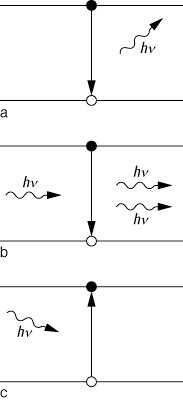
\includegraphics[width=0.2\textwidth]{emission.jpg}
\caption{Laserprinzipien: a) spontane Emission; b) induzierte Emission; c) Absorption.\cite{spektrum}}
\label{fig:emission}
\end{figure}

Findet nun mehr stimulierte Emission statt als Absorption, dann wird immer mehr Licht in Richtung des
bereits vorhandenen Lichts emittiert und das Licht wird immer weiter verstärkt. Dazu müssen sich allerdings mehr Atome im
angeregten als im nicht-angeregten Zustand befinden, da beide Prozesse gleich wahrscheinlich sind. Dieser Zustand wird
Besetzungsinversion genannt.
Er bedeutet jedoch eine Abweichung vom thermodynamischen Gleichgewicht. In diesem befinden sich nämlich mehr Atome im nicht-angeregten
Zustand. Aus diesem Grund muss dem Medium durch sogenanntes Pumpen Energie zugeführt werden.

\begin{figure}
\centering
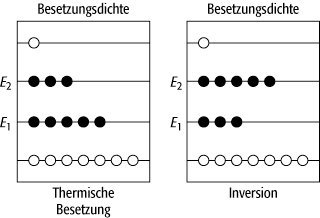
\includegraphics[width=0.4\textwidth]{inversion.jpg}
\caption{Besetzungsdichte bei Inversion im Vergleich zur thermischen Besetzung.\cite{spektrum}}
\label{fig:inversion}
\end{figure}

\subsection{Die Energiepumpe}

Im Glasrohr des Resonators befinden sich zwei Elektroden, an die eine Spannung angelegt wird. Dadurch kommt es im Lasermedium
zur Gasentladung, welche die Heliumatome in einen angeregten Zustand bringt. Durch Stöße übertragen die Heliumatome dann
ihre Energie auf die Neonatome und erzeugen so eine Besetzungsinversion zwischen energetisch hohen und niedrigen
Zuständen.

Das Medium im Laser muss dabei mindstens drei verschiedene Niveaus besetzen können, da in einem 2-Niveau-Laser keine
Besetzungsinversion möglich ist.

\subsection{Die TEM-Moden}

Im Laser sind verschiedene Moden realisierbar, da die Resonanzbedingung $L = n*\lambda/2$ des Resonators von mehreren Wellenlängen
erfüllt werden kann. Die Moden werden dabei als TEM-Moden (Transverse Electromagnetic Modes) bezeichnet. Zwei Zahlen
im Index geben die Ordnung der Moden in x- bzw. y-Richtung an.

Die Intensität der Moden in der einfachsten Ordnung 00 wird durch eine Gaußverteilung beschrieben:

\begin{equation}
  I_{00} = I_0 \text{exp} \biggl(\frac{-2r^2}{\omega^2}\biggr)
\end{equation}

Im He-Ne-Laser mit Brewsterfenstern gilt für alle höheren Ordnungen:

\begin{equation}
  I_{mn} = I_0 \biggl(\frac{\omega_0}{\omega}\biggr)^2 \biggl\lbrack H_m \biggl( \frac{\sqrt(2)x}{\omega} \biggr) \text{exp} \biggl( \frac{-x^2}{\omega^2} \biggr) \biggr\rbrack^2 \biggl\lbrack H_n \biggl( \frac{\sqrt(2)y}{\omega} \biggr) \text{exp} \biggl( \frac{-y^2}{\omega^2} \biggr) \biggr\rbrack^2
\end{equation}

($H$: Hermitesches Polynom, $\omega$: Strahlradius, $\omega_0$: kleinster Strahlradius)

\subsection{Intensität des polarisierten Lichts}

Die Intensität des Lichtes hinter einem Polarisationsfilter lässt sich durch die folgende Formel betimmen.

\begin{equation}
  I = I_0 \text{cos}^2(\delta\phi)
\end{equation}

Dabei ist $I_0$ die Intensität des Lichtes vor dem Filter und $\delta\phi$ der zur Einstellung des Filters verschobene Winkel
der Polarisation des einfallenden Lichtes.

\subsection{Die Wellenlänge des Lasers}

Die Wellenlänge des Lichts wird gemessen, indem ein Gitter in den Strahl gebracht wird. Auf diese Weise treten Interferenzeffekte
auf einem Schirm auf. Mit Hilfe des Abstandes $x$ zwischen dem 0. und dem 1. Hauptmaximum kann die Wellenlänge berechnet werden.

\begin{equation}
  \lambda = g \text{sin}(\text{arctan}(x/d))
\end{equation}

Dabei ist $d$ der Abstand zwischen Schirm und Gitter und $g$ die Gitterkonstante.


\section{Aufbau und Durchführung}

\subsection{Aufbau}
Eine radioaktive Quelle (Am241) wird als $\alpha$-Strahler verwendet. Die emittierten Teilchen werden durch Blenden
kollimiert, sodass sie auf parallelen Bahnen zueinander auf eine dünne Goldfolie treffen. Es wird eine Folie aus Gold
gewählt, da sich dieses Element einfach zu einer dünnen Schicht verarbeiten lässt und eine hohe Atommasse besitzt, sodass
viele Wechselwirkungen stattfinden können.

An der Folie werden die Teilchen
in verschiedene Richtungen bzw. unter verschiedenen Winkeln gestreut, was mit einem Surface-Barrier-Detektor vermessen
werden kann. Der Detektor und ein Verstärker verstärken die aufgenommenen Impulse, die durch auftreffende Teilchen erzeugt
werden. Mit einem Oszilloskop kann eine Energieverlustmessung durchgeführt werden. Des Weiteren steht ein Zähler zur
Verfügung, mit dem Messungen zur Bestimmung des Streuquerschnitts durchgeführt werden können.

Der Aufbau befindet sich in einem Vakuumbehälter, da in diesem Versuch die $\alpha$-Strahlung in Luft lediglich eine
Reichweite von etwa 1,5cm hat.

\begin{figure}
\centering
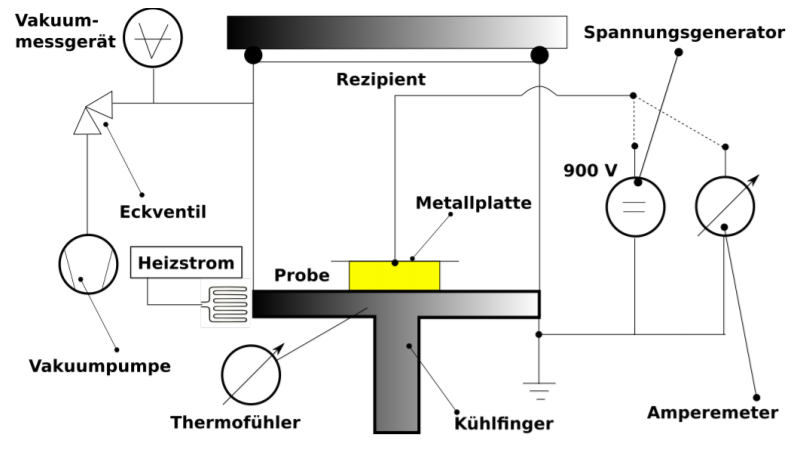
\includegraphics[width=\textwidth]{aufbau.png}
\caption{Schematische Darstellung der Messapparatur \cite[2]{anleitung}.}
\label{fig:aufbau}
\end{figure}


\subsection{Durchführung}
Zunächst wird der Elektromagnet geeicht. Dazu wird mit einer Hallsonde die Abhängigkeit des Magnetfeldes von der Stromstärke
vermessen.

Mit einem Objektiv und der Linse $L_1$ wird das Licht der Cd-Lampe scharf auf den ersten Spalt $S_1$ abgebildet. Die Linse $L_2$
wird so eingestellt, dass ein paralleles Lichtbündel auf das Prisma fällt. Der Duchmesser des Lichtbündels sollte
dabei nicht größer als der des Prismas sein, da ansonsten Strahlungsverluste auftreten.

Mit der Linse $L_3$ wird ein scharfes Bild auf den nächsten Spalt $S_2$ abgebildet. Dieser wird dazu benutzt, eine bestimmte
Wellenlänge auszusuchen. Es wird zuerst die rote Wellenlänge ausgesucht und dann der Polarisationsfilter so eingestellt,
dass nur der $\sigma$-Anteil des Lichtes hindurchgeht.

Die Linse $L_4$ wird so eingestellt, dass sie ein scharfes Bild auf die Lummer-Gehrcke-Platte abbildet.

Das entstehende Interferenzmuster wird mit der Kamera aufgenommen. Es wird dabei ein Bild mit und ein Bild ohne angeschaltetes
Magnetfeld gemacht.

Anschließend wird der blaue Anteil des Spektrums untersucht, wozu der Spalt $S_2$ neu eingestellt wird. Der Polarisationsfilter
wird so eingestellt, dass zunächst der $\sigma$- und anschließend der $\pi$-Anteil betrachtet werden kann.
Ansonsten wird genauso wie bei der roten Linie vorgegangen.


\section{Ergebnisse}
\begin{table}
    \centering
    \caption{Winkelauflösung der Druckamplitude eines Kugelresonator mit 9mm Ring.}
    \label{tab:kugel_ring}
    \begin{tabular}{c c c}
        \toprule
        $\alpha/°$ & $A_{2.146kHz}/\si{\volt}$ & $A_{2.257kHz}/\si{\volt}$\\
        \midrule
        0   &2.57    &2.57\\
        10  &2.61    &2.53\\
        20  &2.61    &2.45\\
        30  &2.65    &2.25\\
        40  &2.57    &2.01\\
        50  &2.53    &1.29\\
        60  &2.53    &1.29\\
        70  &2.49    &0.92\\
        80  &2.45    &0.45\\
        90  &2.45    &0.067\\
        100 &2.53    &0.44\\
        110 &2.53    &0.87\\
        120 &2.57    &1.35\\
        130 &2.61    &1.69\\
        140 &2.61    &2.01\\
        150 &2.57    &2.25\\
        160 &2.57    &2.53\\
        170 &2.53    &2.61\\
        180 &2.53    &2.69\\
        \bottomrule
    \end{tabular}
\end{table}

\begin{table}
    \centering
    \caption{Resonanzfrequenzen des Kugelresonators}
    \label{tab:kugel_resonanz}
    \begin{tabular}{c c c}
        \toprule
        $f/\si{\kilo\hertz}$ & $A/\si{\volt}$ & $\phi/°$\\
        \midrule
        0.410   &0.2     &96\\
        2.286   &3.3     &-71\\
        3.666   &9.6     &77\\
        4.940   &7.6     &-80\\
        6.174   &11.1    &41\\
        7.379   &10.5    &-143\\
        7.983   &6       &19\\
        8.564   &8.4     &-5\\
        9.395   &7       &158\\
        9.733   &7.1     &146\\
        \bottomrule
    \end{tabular}
\end{table}

\begin{table}
    \centering
    \caption{Resonanzfrequenzen des Kugelresonators}
    \label{tab:kugel_resonanz_winkel}
    \begin{tabular}{c c c c}
        \toprule
        $\alpha/°$ & $A_{3,666kHz}/\si{\volt}$ & $A_{6,174kHz}/\si{\volt}$ & $A_{7,379kHz}/\si{\volt}$ \\
        \midrule
        0   &5.9     &1.21    &0.082\\
        10  &5.3     &1.25    &0.285\\
        20  &5.1     &2.53    &0.52\\
        30  &4.9     &3.46    &1.33\\
        40  &4.9     &3.7     &1.91\\
        50  &4.4     &3.54    &2.85\\
        60  &2.3     &2.65    &3.54\\
        70  &2.7     &1.25    &3.66\\
        80  &2.4     &0.9     &2.93\\
        90  &1.6     &3.34    &1.25\\
        100 &0.64    &4.94    &1.13\\
        110 &1.21    &5.87    &3.54\\
        120 &2.65    &5.31    &4.7\\
        130 &4.4     &3.42    &4.3\\
        140 &5.5     &0.374   &2.01\\
        150 &7.1     &3.5     &1.93\\
        160 &7.7     &7       &6.1\\
        170 &8.7     &9.3     &8.5\\
        180 &8.8     &10.1    &9.8\\
        \bottomrule
    \end{tabular}
\end{table}

\begin{table}
    \centering
    \caption{Resonanzfrequenzen des gekoppelten Kugelresonators}
    \label{tab:molekül}
    \begin{tabular}{c c c}
        \toprule
        $\alpha/°$ & $A_{2,256kHz}/\si{\volt}$ & $A_{2,327kHz}/\si{\volt}$\\
        \midrule
        0   &1.73    &1.51\\
        10  &1.71    &1.53\\
        20  &1.73    &1.53\\
        30  &1.73    &1.49\\
        40  &1.71    &1.53\\
        50  &1.71    &1.53\\
        60  &1.65    &1.53\\
        70  &1.65    &1.53\\
        80  &1.67    &1.53\\
        90  &1.67    &1.53\\
        100 &1.67    &1.53\\
        110 &1.69    &1.53\\
        120 &1.67    &1.53\\
        130 &1.67    &1.53\\
        140 &1.67    &1.53\\
        150 &1.67    &1.53\\
        160 &1.67    &1.53\\
        170 &1.67    &1.53\\
        180 &1.67    &1.53\\
        \bottomrule
    \end{tabular}
\end{table}

\begin{table}
    \centering
    \caption{Resonanzfrequenzen des gekoppelten Kugelresonators}
    \label{tab:zylinder}
    \begin{tabular}{c c c c c c c}
        \toprule
        $L/\si{\milli\meter}$ & $F_1/\si{\kilo\hertz}$ & $\phi_1/°$ & $A_1/\si{\volt}$ & $F_2/\si{\kilo\hertz}$ & $\phi_2/°$ & $A_2/\si{\volt}$\\
        \midrule
        50  &6.83    &37      &6.03    &10.206  &141     &3.58\\
        75  &6.84    &-137    &5.31    &9.106   &-3      &4.10\\
        100 &6.843   &37.5    &4.42    &8.546   &-175    &3.82\\
        125 &6.856   &-145    &3.74    &8.219   &10      &3.62\\
        150 &6.855   &31.2    &3.22    &7.998   &-178    &2.73\\
        175 &6.859   &-140.4  &2.97    &7.829   &20.8    &3.02\\
        200 &6.856   &40      &2.57    &7.708   &-158    &2.73\\
        250 &6.856   &36      &2.03    &7.539   &-154    &2.27\\
        300 &6.853   &34.5    &1.95    &7.425   &-150    &2.03\\
        350 &6.853   &39      &1.83    &7.345   &-150    &1.85\\
        400 &6.854   &38      &1.63    &7.283   &-145.1  &1.67\\
        450 &6.855   &36      &1.46    &7.238   &-147.4  &1.51\\
        \bottomrule
    \end{tabular}
\end{table}

\section{Auswertung}
\subsection{Untergrundsubtraktion}
Es wird ein exponentieller Untergrund angenommen.
\begin{equation}
  I_{Untergrund}(T) = ae^{bT}+c
\end{equation}
Mit den Daten aus Tabelle \ref{tab:2grad} ergeben sich für die $2\si{\kelvin\per\minute}$-Heizrate die Parameter
\begin{align}
  a &= (7,88\pm 2,38)\SI{e-2}{\pico\ampere} \nonumber\\
  b &= (1,74\pm 0,09)\SI{e-2}{\per\kelvin} \nonumber\\
  c &= (-3,27\pm 0,42)\si{\pico\ampere}
\end{align}
und aus Tabelle \ref{tab:1,5grad} für die die $1,5\si{\kelvin\per\minute}$-Heizrate die Parameter
\begin{align}
  a &= (1,48\pm 0,78)\si{\pico\ampere} \nonumber\\
  b &= (7,00\pm 1,25)\SI{e-3}{\per\kelvin} \nonumber\\
  c &= (-6,49\pm 1,75)\si{\pico\ampere}
\end{align}
Die Messwerte und die Ausgleichskurven sind in Abbildung \ref{fig:Mit_Untergrund} und die bereinigten Werte in Abbildung \ref{fig:Bereinigt} dargestellt.
\begin{figure}
  \centering
  \begin{subfigure}{0.4\textwidth}
    \centering
    \includegraphics[width=\textwidth]{build/I_mit_untergrund_2.pdf}
    \subcaption{Heizrate von $2\si{\kelvin\per\minute}$}
  \end{subfigure}
  \begin{subfigure}{0.4\textwidth}
    \centering
    \includegraphics[width=\textwidth]{build/I_mit_untergrund_15.pdf}
    \subcaption{Heizrate von $1,5\si{\kelvin\per\minute}$}
  \end{subfigure}
  \caption{Gemessener Strom. In die Ausgleichsrechnung miteinbezogene Werte sind in schwarz.}
  \label{fig:Mit_Untergrund}
\end{figure}

\begin{figure}
  \centering
  \begin{subfigure}{0.4\textwidth}
    \centering
    \includegraphics[width=\textwidth]{build/I_2.pdf}
    \subcaption{Heizrate von $2\si{\kelvin\per\minute}$}
  \end{subfigure}
  \begin{subfigure}{0.4\textwidth}
    \centering
    \includegraphics[width=\textwidth]{build/I_15.pdf}
    \subcaption{Heizrate von $1,5\si{\kelvin\per\minute}$}
  \end{subfigure}
  \caption{Bereinigter Strom}
  \label{fig:Bereinigt}
\end{figure}

\subsection{Aktivierungsarbeit aus Anlaufkurve}
Da der erste Berg als eine Exponentialfunktion ist ergibt sich die Beziehung
\begin{equation}
  \text{ln}(I(T)) = \frac{-W}{k_bT} + b
\end{equation}
Es lassen sich aus den bereinigten Daten die Werte
\begin{align}
  W &= (1,260\pm 0,084)\SI{e-19}{\joule}\nonumber\\
  b &= 38,0\pm 2,4
\end{align}
für die $2\si{\kelvin\per\minute}$-Heizrate und
\begin{align}
  W &= (6,87\pm 0,84)\SI{e-20}{\joule}\nonumber\\
  b &= 21,5\pm 2,4
\end{align}
für die $1,5\si{\kelvin\per\minute}$-Heizrate bestimmen.
Die Werte sind in Abbildung \ref{fig:Anlauf} dargestellt.

\begin{figure}
  \centering
  \begin{subfigure}{0.4\textwidth}
    \centering
    \includegraphics[width=\textwidth]{build/Anlauf_2.pdf}
    \subcaption{Heizrate von $2\si{\kelvin\per\minute}$}
  \end{subfigure}
  \begin{subfigure}{0.4\textwidth}
    \centering
    \includegraphics[width=\textwidth]{build/Anlauf_15.pdf}
    \subcaption{Heizrate von $1,5\si{\kelvin\per\minute}$}
  \end{subfigure}
  \caption{Logarithmierter Strom gegenüber inverser Temperatur}
  \label{fig:Anlauf}
\end{figure}

\subsection{Aktivierungsarbeit aus Integration}
Die Funktion ist ebenfalls exponentialverteilt, bzw.
\begin{equation}
  \text{ln}(f(T)) = \frac{-W}{k_bT} + b
\end{equation}
es ergeben sich die Werte
\begin{align}
  W &= (1,721\pm 0,028)\SI{e-19}{\joule}\nonumber\\
  b &= -46,7\pm 0,8
\end{align}
für die $2\si{\kelvin\per\minute}$-Heizrate und
\begin{align}
  W &= (1,872\pm 0,105)\SI{e-19}{\joule}\nonumber\\
  b &= -51,4\pm 3,0
\end{align}
für die $1,5\si{\kelvin\per\minute}$-Heizrate bestimmen.
Die Werte sind in Abbildung \ref{fig:Integriert} dargestellt.

\begin{figure}
  \centering
  \begin{subfigure}{0.4\textwidth}
    \centering
    \includegraphics[width=\textwidth]{build/Integriert_2.pdf}
    \subcaption{Heizrate von $2\si{\kelvin\per\minute}$}
  \end{subfigure}
  \begin{subfigure}{0.4\textwidth}
    \centering
    \includegraphics[width=\textwidth]{build/Integriert_15.pdf}
    \subcaption{Heizrate von $1,5\si{\kelvin\per\minute}$}
  \end{subfigure}
  \caption{$\text{ln}(f(T))$ gegenüber inverser Temperatur}
  \label{fig:Integriert}
\end{figure}


\section{Diskussion}
\begin{table}
    \centering
    \caption{Vergleich gemessener und berechneter Werte der Lande-Faktoren}
    \label{tab:Endergebnisse}
    \begin{tabular}{ccc}
        \toprule
        Linie & $g_{j,theorie}$ & $g_{j,gemessen}$\\
        \midrule
        rot             & $1$       & $0,970\pm 0,022$\\
        blau($\sigma$)  & $0,5$     & $0,548\pm 0,010$\\
        blau($\pi$)     & $1,75$    & $1,78\pm 0,06$\\
        \bottomrule
    \end{tabular}
\end{table}
Die theoretisch berechneten Lande-Faktoren befinden sich innerhalb oder nahe an den gemessenen Werten mit ihren Fehlerintervallen.
Bedenkt man hierzu noch, dass die Ableseunsicherheiten der $\Delta s$ und $\delta s$ nicht mit in die Rechnung eingingen,
und die Kamera zwischen Bildern sich minimal bewegt, kann die Theorie hier zumindest annähernd bestätigt werden.

\newpage
\nocite{*}
\printbibliography

\end{document}
